%!TEX root=../../autopilot.tex
\section{Agents}
\label{sec:agents}

All of Autopilot's components can be organized into a single system as an "agent," the executable that coordinates everyday use. An agent encapsulates:

\begin{itemize}
\item \textbf{Runtime Logic} --- an initialization routine that starts any needed system processes and any subsequent operations that define the behavior of the agent.
\item \textbf{Networking Station} --- Agents have networking objects called \texttt{Station}s that are intended to be the "load bearing" networking objects (described more \hyperref[sec:networking]{below}).
\item \textbf{Callbacks} --- An action vocabulary that maps different types of messages to methods for handling them. Called \texttt{listens} to disambiguate from other types of callbacks.
\item \textbf{Dependencies} --- Required packages, libraries, and system reconfigurations needed to operate. Python dependencies are currently defined for agents as groups of \href{https://peps.python.org/pep-0621/\#dependencies-optional-dependencies}{optional packages}\sidenote{As of v0.5.0, Autopilot is packaged with \href{https://python-poetry.org}{Poetry}, so they are \texttt{[tool.poetry.extras]} entries within the \texttt{pyproject.toml} file, installed with pip like \texttt{pip install auto-pi-lot[pilot]} or poetry like \texttt{poetry install -E pilot}}, and system configuration is done with \href{https://docs.auto-pi-lot.com/en/latest/setup/scripts.html}{scripts} which shorthand common operations like \href{https://github.com/auto-pi-lot/autopilot/blob/90956187d4222f16f67ab8b39b8359da954d5dcc/autopilot/setup/scripts.py\#L140-L183}{compiling OpenCV} with optimizations for the raspi or \href{https://github.com/auto-pi-lot/autopilot/blob/90956187d4222f16f67ab8b39b8359da954d5dcc/autopilot/setup/scripts.py\#L92-L100}{enabling a soundcard}.
\end{itemize}

Together, these define an agent's \textit{role} in the swarm.

\clearpage

There are currently two agents in Autopilot: 

\begin{itemize}
    \item \textbf{Terminal} - The user-facing control agent.
    \item \textbf{Pilot} - A Raspberry Pi that runs tasks, coordinates hardware, and optionally coordinates a set of child Pis.
\end{itemize}



\textbf{Terminal}\marginnote[-0.25cm]{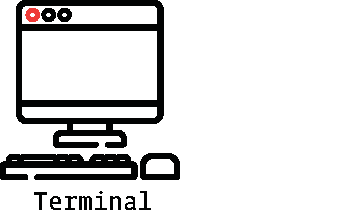
\includegraphics[]{figures/side_27_terminal.pdf}} agents serve as a root node (see Section \ref{sec:networking}) in an Autopilot swarm. The terminal is the only agent with a \hyperref[sec:ui]{GUI}, which is used to control its connected pilots and visualize incoming task data. The terminal also manages data and keeps a registry of all active experimental subjects. The terminal is intended to make the day-to-day use of an Autopilot swarm manageable, even for those without programming experience. The terminal GUI is described further in Section \ref{sec:ui}.

\textbf{Pilot}\marginnote{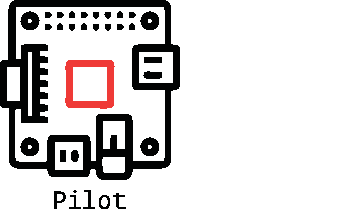
\includegraphics[]{figures/side_28_pilot.pdf}} agents are the workhorses of Autopilot---the agents that run the experiments. Pilots are intended to operate as always-on, continuously running system services. Pilots make a network connection to a terminal and wait for further instructions. They maintain the system-level software used for interfacing with the hardware connected to the Raspberry Pi, receive and execute tasks, and continually return data to the terminal for storage.

Each agent runs autonomously, and so a Pilot can run a task without a Terminal and store data locally, a Terminal can be used without Pilots to define protocols and manage subjects, and so on. This decoupling lets each agent have more freedom in its behavior at the expense of the complexity of configuring and maintaining them (see Sec. \ref{future:knowledge} and \ref{future:metastructure}). All interaction is based on the "listen" callbacks known by the agents, so to start a task a Terminal will send a Pilot a \texttt{"START"} message containing information about a \texttt{Task} class that it is to run along with its parameterization. The Pilot then attempts to run the task, sends a message to the Terminal alerting it to a \texttt{"STATE"} change, and begins streaming data back to it in messages with a \texttt{"DATA"} key.

Each\marginnote[-0.5cm]{
\includegraphics[]{figures/side_29_child.pdf}} pilot is capable of mutually coordinating with one or many \textbf{Copilots}\sidenote{A previous version of this paper described a third, subordinate "Child" agent that performed auxiliary operations in a task. We now view such a hierarchy as unnecessary, and that distribution of labor within a task is better served by a fluid combination of multiple Pilots than thinking of them as qualitatively different agents. We now refer one among multiple agents performing a task together as a "copilot."}. We are still experimenting with, and thus openminded to the best way to structure multi-pilot tasks. Like many things in Autopilot, there is no one right way to do it, and the strategy depends on the particular constraints of the task. We include a few examples in the network latency and go/no-go tasks in the \href{https://wiki.auto-pi-lot.com/index.php/Plugin:Autopilot\_Paper}{plugin} that accompanies this paper, and expand on this a bit further in a few parts of section \ref{sec:future}, as it is a major point of active development.


\subsection{Behavioral topologies}
\label{sec:topology}

We think one of the most transformative features of Autopilot's distributed structure is the control that users have over what we call "behavioral topology." The logic of hardware and task operation within an agent, the distribution of labor between agents performing a task, and the pattern of connectivity and command within a swarm of agents constitute a topology. 

Below we illustrate this idea with a few examples:

\clearpage

\begin{itemize}
    \item \textbf{Pilot Swarm}\marginnote{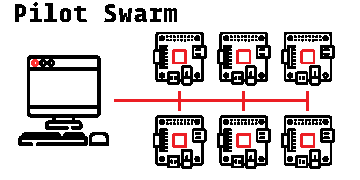
\includegraphics[]{figures/side_20_swarm.pdf}} - The first and most obvious topological departure from traditional behavioral instrumentation is the use of a single computer to independently coordinate tasks in parallel. Our primary installation of Autopilot is a cluster of 10 behavior boxes that can independently run tasks dispatched from a central terminal which manages data and visualization. This topology highlights the expandability of an Autopilot system: adding new pilots is inexpensive, and the single central terminal makes controlling experiments and managing data simple.
    \item \textbf{Shared Task} - \marginnote{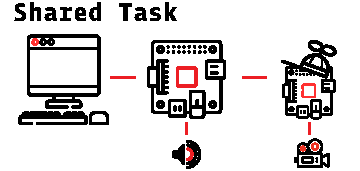
\includegraphics[]{figures/side_21_shared.pdf}} Tasks can be shared across a set of copilots to handle tasks with computationally intensive operations. For example, in an open-field navigation task, one pilot can deliver position-dependent sounds while another records and analyzes video of the arena to track the animal's position. The terminal only needs to be configured to connect to the parent pilot, but the other copilot is free to send data to the Terminal marked for storage in the subject's file as well.
    \item \textbf{Distributed Task}\marginnote{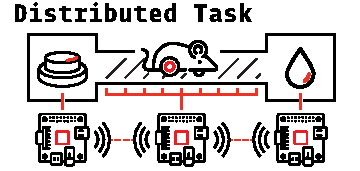
\includegraphics[]{figures/side_22_distributed.pdf}} - Many pilots with overlapping responsibilities can cooperate to perform distributed tasks. We anticipate this will be useful when the experimental arenas can't be fully contained (such as natural environments), or when experiments require simultaneous input and output from multiple subjects. Distributed tasks can take advantage of the Pi's wireless communication, enabling, for example, experiments that require many networked cameras to observe an area, or experiments that use the Pis themselves as an interface in a multisubject augmented reality experiment.
    \item \textbf{Multi-Agent Task}\marginnote{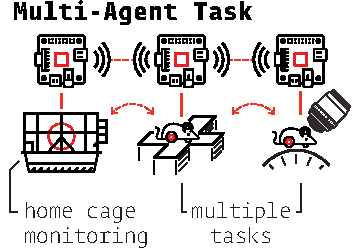
\includegraphics[]{figures/side_23_multi.pdf}} - Neuroscientific research often consists of multiple mutually interdependent experiments, each with radically different instrumentation. Autopilot provides a framework to unify these experiments by allowing users to rewrite core functionality of the program while maintaining integration between its components. For example, a neuroethologist could build a new \hyperref[sec:futureagents]{"Observer"} agent that continually monitors an animal's natural behavior in its home cage to calibrate a parameter in a task run by a pilot. If they wanted to manipulate the behavior, they could build a "Compute" agent that processes Calcium imaging data taken while the animal performs the task to generate and administer patterns of optogenetic stimulation. Accordingly, passively observed data can be combined with multiple experimental datasets from across the subject's lifespan. We think that unifying diverse experimental data streams with interoperable frameworks is the best way to perform experiments that measure natural behavior in the fullness of its complexity in order to understand the naturally behaving brain\citep{dattaComputationalNeuroethologyCall2019}.
\end{itemize}
